\documentclass[german,11pt]{beamer}
% ------------------------------------------------------------------------------
% Packages
\usepackage[german,english,french]{babel}
\usepackage[T1]{fontenc}
\usepackage[utf8]{inputenc}
\usepackage{ragged2e}
\usepackage[normalem]{ulem}


\usepackage{listings}
\usepackage{color}
\usepackage{xcolor} 
\usepackage{plantuml}
% \usepackage{enumitem} \setitemize{leftmargin=*}   // Keine Aufzählung
\usepackage{pgfplots}

\usepackage{csquotes}

\pgfplotsset{compat=1.18}

\definecolor{dkgreen} {rgb}{0,0.6,0}
\definecolor{gray}{rgb}{0.5,0.5,0.5}
\definecolor{mauve}{rgb}{0.58,0,0.82}

\lstset{frame=tb,
  language=Java,
  aboveskip=3mm,
  belowskip=3mm,
  showstringspaces=false,
  columns=flexible,
  basicstyle={\small\ttfamily},
  numbers=none,
  numberstyle=\tiny\color{gray},
  keywordstyle=\color{blue},
  commentstyle=\color{dkgreen},
  stringstyle=\color{mauve},
  breaklines=true,
  breakatwhitespace=true,
  tabsize=3
}
% ------------------------------------------------------------------------------
% Parameters
\mode<presentation>{\usetheme{Luebeck}}
\setbeamertemplate{itemize items}[triangle]
\setbeamercovered{transparent}
\usecolortheme{dove}
\usefonttheme{serif}
\addtobeamertemplate{block begin}{}{\justifying}
% ToC
\AtBeginSection[] {
  \begin{frame}{Inhalt}
    \tableofcontents[currentsection]
  \end{frame}
}
% Headline
\makeatletter
\setbeamertemplate{headline}{%
  \leavevmode%
  \@tempdimb=2.4375ex%
  \ifnum\beamer@subsectionmax<\beamer@sectionmax%
    \multiply\@tempdimb by\beamer@sectionmax%
  \else%
    \multiply\@tempdimb by\beamer@subsectionmax%
  \fi%
  \ifdim\@tempdimb>0pt%
    \advance\@tempdimb by 1.825ex%
    \begin{beamercolorbox}[wd=.5\paperwidth,ht=\@tempdimb]{section in head/foot}%
      \vbox to\@tempdimb{\hfill\insertsectionnavigation{.3\paperwidth}\vfil}%
    \end{beamercolorbox}%
    \begin{beamercolorbox}[wd=.3\paperwidth,ht=\@tempdimb]{subsection in head/foot}%
      \vbox to\@tempdimb{\vfil\insertsubsectionnavigation{.5\paperwidth}\vfil}%
    \end{beamercolorbox}%
    \begin{beamercolorbox}[wd=.2\paperwidth,ht=\@tempdimb]{subsection in head/foot}%
      \vbox to\@tempdimb{\vfil\hfill
\includegraphics[height=1cm]{fig/graphics/logo.jpg}\vfil}
    \end{beamercolorbox}%    
  \fi%
}
\makeatother
% Footline
\makeatletter
\setbeamertemplate{footline}{%
  \leavevmode%
  \hbox{\begin{beamercolorbox}[wd=.5\paperwidth,ht=2.5ex,dp=1.125ex,leftskip=.3cm,rightskip=.3cm]{author in head/foot}%
    \usebeamerfont{author in head/foot}\insertshortdate \hfill \insertshortauthor
  \end{beamercolorbox}%
  \begin{beamercolorbox}[wd=.5\paperwidth,ht=2.5ex,dp=1.125ex,leftskip=.3cm,rightskip=.3cm plus1fil]{title in head/foot}%
    \usebeamerfont{title in head/foot}\insertshorttitle \hfill \insertframenumber\,/\,\inserttotalframenumber
  \end{beamercolorbox}}%
  \vskip0pt%
}
\makeatother

\addto\captionsenglish{% Replace "english" with the language you use
  \renewcommand{\contentsname}%
    {Whatever}%
}

% ------------------------------------------------------------------------------
% Infos
\title[VS]{Verteilte Systeme}
%\subtitle[Short subtitle]{Subtitle}
\author[BCK]{Prof. Dr. Martin Becke}
\date[0.9]{Version 0.9}
\institute[CaDS]{CaDS - HAW Hamburg}
%\logo{
\includegraphics[height=1cm]{fig/graphics/logo.jpg}}
% ------------------------------------------------------------------------------

% Document
\begin{document}

% ------------------------------------------------------------------------------
% Titlepage
\begin{frame}
  \titlepage{}
\end{frame}
% ------------------------------------------------------------------------------
% ToC
%\begin{frame}{Contents}
%  \tableofcontents
%\end{frame}
% ------------------------------------------------------------------------------
\section{Supporting Patterns I}

\subsection{Model Viewer Controller}
\begin{frame}
  \frametitle{Model Viewer Controller (MVC)}
  \framesubtitle{Idee}
  \begin{itemize}
    \item Sowohl Entwurfsmuster, also auch Designentwurf
    \item Hier Konzentration auf MVC-Architekturmuster
    \item Besteht aus drei Hauptkomponenten 
    \item Klare Trennung im Modell kann Aufwände verursachen (JavaFX) -> Siehe Beispiel
  \end{itemize}
\end{frame}

\begin{frame}
  \frametitle{Model Viewer Controller (MVC)}
  \framesubtitle{Struktur}
  \begin{figure}[ht]
    \centering
    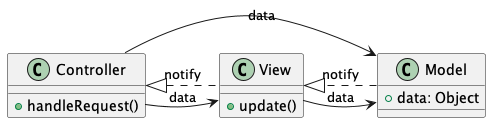
\includegraphics[width=0.7\textwidth]{fig/uml/default-mvc.png}
    \caption{Beispiel eines Basis MVC Architekturmusters}
    \label{fig:default-mvc}
  \end{figure}
\end{frame}

\begin{frame}
  \frametitle{Model Viewer Controller (MVC)}
  \framesubtitle{Fallbeispiel Led-Lampe}
  \begin{itemize}
    \item Mobile-App (Android Node) 
    \item Node.js Instanz (PI)
    \item Smarte Lampe  (Leuchtmittel mit ESP32) 
  \end{itemize}
\end{frame}

\begin{frame}
  \frametitle{Model Viewer Controller (MVC)}
  \framesubtitle{Struktur}
  \begin{figure}[ht]
    \centering
    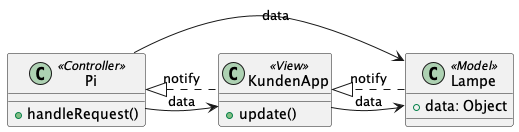
\includegraphics[width=0.7\textwidth]{fig/uml/sterotypen-mvc.png}
    \caption{MVC Architekturmusters im Fallbeispiel mit Sterotypen}
    \label{fig:stereo-mvc}
  \end{figure}
\end{frame}

\begin{frame}
  %\frametitle{Model Viewer Controller (MVC)}
  \framesubtitle{In Schichten: VCM und CVM}
  \begin{figure}[ht]
    \centering
    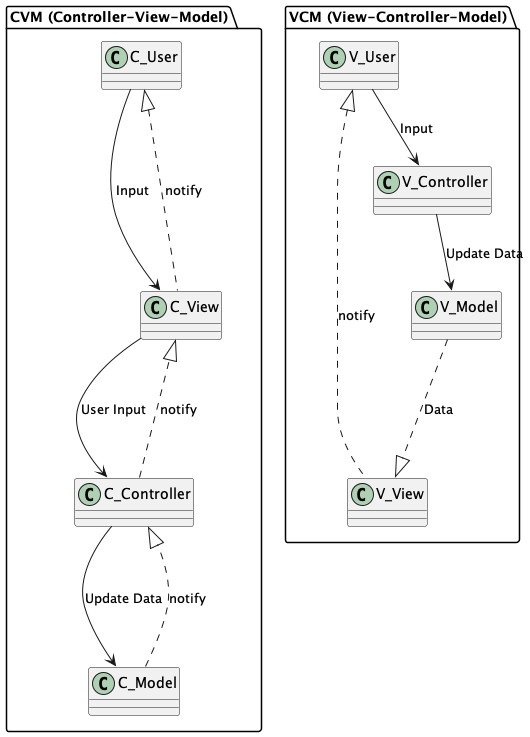
\includegraphics[width=0.40\textwidth]{fig/uml/mvc-varianten.png}
    \caption{Mögliche Varianten vom MVC in Schichten gedacht}
    \label{fig:mvs-varianten}
  \end{figure}
\end{frame}


\begin{frame}[fragile]
\begin{table}[ht]
\noindent\begin{minipage}[b]{1\linewidth}\centering
\begin{lstlisting}[caption={Java FX Input},captionpos=b,label={lst:javafx-input}]
public class JavaFXUserInputExample extends Application {

    public static void main(String[] args) {
        launch(args);
    }

    @Override
    public void start(Stage primaryStage) {
        Button button = new Button("Click me!");

        // Registering an EventHandler for the button click
        button.setOnAction(event -> {
            System.out.println("Button clicked!");
        });

        StackPane root = new StackPane();
        root.getChildren().add(button);

        Scene scene = new Scene(root, 300, 250);

        primaryStage.setTitle("JavaFX User Input Example");
        primaryStage.setScene(scene);
        primaryStage.show();
    }
}
\end{lstlisting}
\end{minipage}
\end{table}
\end{frame}

\subsection{Vertreter}
\begin{frame}
  \frametitle{Proxy}
  \framesubtitle{Idee}
  \begin{itemize}
    \item Zwischen Consumer und Provider platziert
    \item Ein Platzhalter, ein Vermittler
    \item Kann mit Caching Netzwerklatenz reduzieren
    \item Kann die Sicherheit erhöhen
  \end{itemize}
\end{frame}

\begin{frame}
  \frametitle{Proxy}
  \framesubtitle{Design als Pattern}
\begin{figure}[ht]
  \centering
  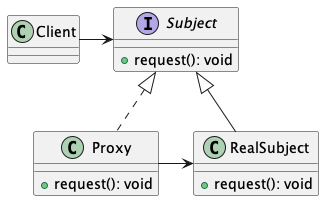
\includegraphics[width=0.45\textwidth]{fig/uml/proxy.png}
  \caption{Proxy Pattern}
  \label{fig:proxy}
\end{figure}
\end{frame}

\begin{frame}
  \frametitle{Proxy}
  \framesubtitle{Typen}
  \begin{itemize}
    \item Forward Proxy
    \item Reverse Proxy
    \item Caching Proxy
    \item Load Balancing Proxy
  \end{itemize}
\end{frame}

\begin{frame}
  \frametitle{Broker}
  \framesubtitle{Idee}
  \begin{itemize}
    \item Zwischen Consumer und Provider platziert
    \item Ein Vermittler mit erweiterten Funktionen
    \item Kann Nachrichten filtern, transformieren und aggregieren
    \item Unterstützt mehrere Protokolle
    \item Kann über eine Warteschlange für eine asynchrone Auslieferung verfügen
  \end{itemize}
\end{frame}

\begin{frame}
  \frametitle{Broker}
  \framesubtitle{Design als Pattern}
\begin{figure}[ht]
  \centering
  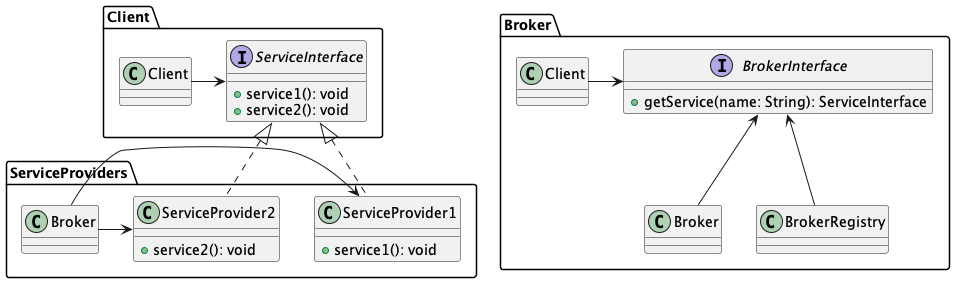
\includegraphics[width=1\textwidth]{fig/uml/broker.png}
  \caption{Broker Pattern}
  \label{fig:broker}
\end{figure}
\end{frame}

\begin{frame}
  \frametitle{Broker}
  \framesubtitle{Typen}
  \begin{itemize}
    \item Forwarding-Broker
    \item Handle-Driven-Broker 
  \end{itemize}
\end{frame}

\begin{frame}
  \frametitle{Trader}
  \framesubtitle{Idee}
  \begin{itemize}
    \item Zwischen Consumer und Provider platziert
    \item Ein Vermittler mit eigener Entscheidungskompetenz
    \item Kann Katalog von Diensten nach Kriterien anbieten
  \end{itemize}
\end{frame}
%\section{Einleitung}
\subsection{Observer}
\begin{frame}
  \frametitle{Observer}
  \framesubtitle{Idee}
  \begin{itemize}
    \item Lösung für unmittelbare Kommunikation
    \item $1:n$-Beziehung zwischen Objekten 
    \item Benachrichtigt, wenn sich sein Zustand ändert (Event)
    \item Ermöglicht eine lose Kopplung im Design
    \item Erhält enge Kopplung in der Kommunikation
  \end{itemize}
\end{frame}

\begin{frame}
  %\frametitle{Observer}
  \framesubtitle{Pattern}
  \begin{figure}[ht]
    \centering
    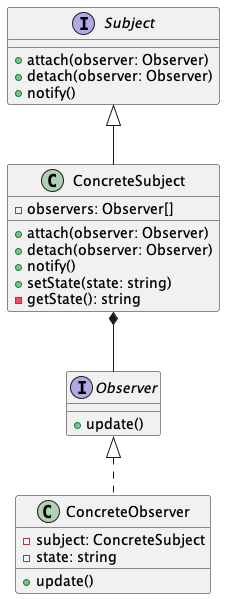
\includegraphics[width=0.18\textwidth]{fig/uml/default-observer.png}
    \caption{Einfaches Observer Pattern}
    \label{fig:default-observer}
  \end{figure}
\end{frame}

\begin{frame}
  %\frametitle{Observer}
  \framesubtitle{Pattern Beispiel Lampe - Architektur}
  \begin{figure}[ht]
    \centering
    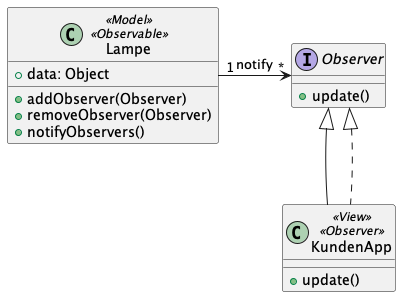
\includegraphics[width=0.65\textwidth]{fig/uml/mvc-observer.png}
    \caption{Observer Pattern als Verbindung zwischen Model und View}
    \label{fig:mvc-observer}
  \end{figure}
\end{frame}

\begin{frame}
  \frametitle{Observer}
  \framesubtitle{Pattern Beispiel Lampe - Verhalten}
  \begin{figure}[ht]
    \centering
    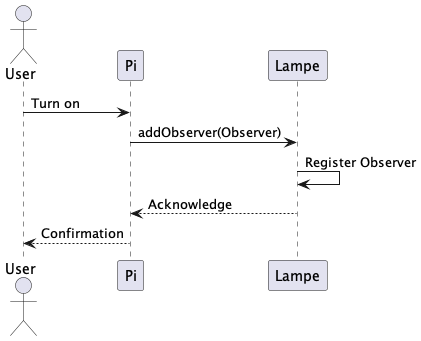
\includegraphics[width=0.55\textwidth]{fig/uml/seq-mvc-observer.png}
    \caption{Observer Pattern als Verbindung zwischen Model und View}
    \label{fig:seq-mvc-observer}
  \end{figure}
\end{frame}

\begin{frame}
  \frametitle{Observer}
  \framesubtitle{Im Kontext von MVC und VS}
  \begin{itemize}
    \item Nicht nur eine Design-Frage
    \item Technologie-abhängig
    \item Uni-direktionalen Kommunikation zwischen dem Subjekt und den Beobachtern
    \item Request-Response-Cycle unterstützt Observer nicht direkt
    \item WebSockets, Long Polling, HTTP2 oder HTTP3 können Optionen anbieten
  \end{itemize}
\end{frame}
%\section{Einleitung}
\subsection{Callback}
\begin{frame}
  \frametitle{Callback}
  \framesubtitle{Idee}
  \begin{itemize}
    \item Funktion (Methode oder Prozedur) als Argument an eine andere Funktion
    \item Nach Abschluss einer bestimmten Aufgabe wird Funktion ausgeführt
    \item Aufrufende Funktion muss nichts vom Callback wissen
    \item Kommunikation unidirektional
    \item Callback-Pattern wird häufig in der asynchronen Programmierung verwendet
    \item Callback-Pattern eignet sich gut für ereignisgesteuerte Programmierung
  \end{itemize}
\end{frame}

\begin{frame}
  \frametitle{Callback}
  \framesubtitle{Callback Pattern}
  \begin{figure}[!ht]
    \centering
    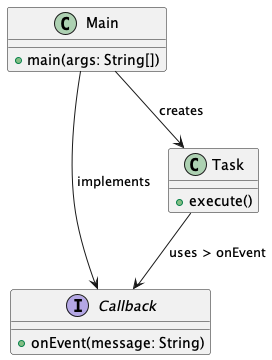
\includegraphics[width=0.35\textwidth]{fig/uml/callback-class.png}
    \caption{Callback Pattern}
    \label{fig:callback-class}
  \end{figure}
\end{frame}

\begin{frame}
  \frametitle{Callback}
  \framesubtitle{Callback Pattern Sequenz}
  \begin{figure}[!ht]
    \centering
    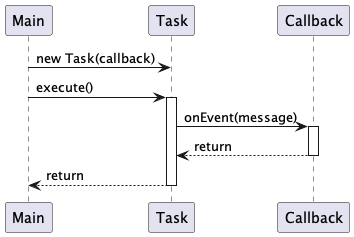
\includegraphics[width=0.65\textwidth]{fig/uml/callback-seq.png}
    \caption{Callback Pattern Sequenz}
    \label{fig:callback-seq}
  \end{figure}
\end{frame}

%\section{Einleitung}
\subsection{Singleton}
\begin{frame}
  \frametitle{Singleton}
  \framesubtitle{Idee}
  \begin{itemize}
    \item Klasse hat nur eine einzige Instanz
    \item Globalen Zugriffspunkt zu dieser Instanz
  
  \end{itemize}
\end{frame}

\begin{frame}
  \frametitle{Singleton}
  \framesubtitle{Pattern}
  \begin{figure}[!ht]
    \centering
    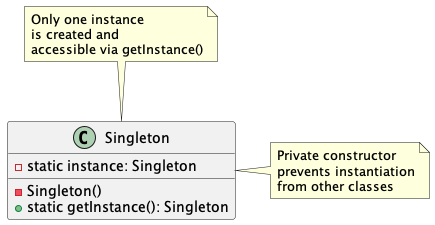
\includegraphics[width=0.65\textwidth]{fig/uml/singleton.png}
    \caption{Singleton Pattern}
    \label{fig:singleton}
  \end{figure}
\end{frame}

\begin{frame}
  \frametitle{Singleton}
  \framesubtitle{Diskussion Eignung}
  \begin{itemize}
    \item Herausforderung in VS, insbesondere bei gleichzeitigen Zugriff
    \item Nutzen spezifischen Anforderungen
    \item Manchmal sinnvoll: Zentrale Verwalten von Ressourcen und die Steuerung eines globalen Zustands
    \item Alternativen prüfen
  \end{itemize}
\end{frame}
%\section{Einleitung}
\subsection{Factory}
\begin{frame}
  \frametitle{Factory}
  \framesubtitle{Idee}
  \begin{itemize}
    \item Objekterstellung mittels separater Klasse
    \item Kann Client-Code von den konkreten Implementierungsdetails entkoppeln
    \item Verschiedene Implementierungen können unterstützt werden
    \item Kann Komplexität kapseln
    \item Ressourcen können zentral erstellt und verwaltet werden
    \item Kann Load Balancing und Failover-Mechanismen implementieren
  \end{itemize}
\end{frame}


\begin{frame}
  \frametitle{Factory}
  \framesubtitle{Pattern}
  \begin{figure}[!ht]
    \centering
    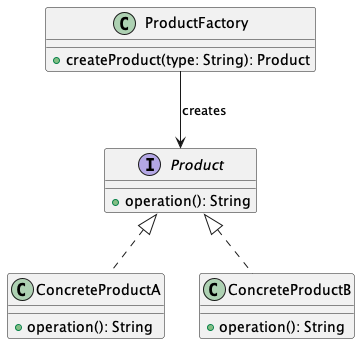
\includegraphics[width=0.45\textwidth]{fig/uml/factory-class.png}
    \caption{Factory Pattern}
    \label{fig:factory-class}
  \end{figure}
\end{frame}

\begin{frame}
  \frametitle{Factory}
  \framesubtitle{Sequenz}
   \begin{figure}[!ht]
    \centering
    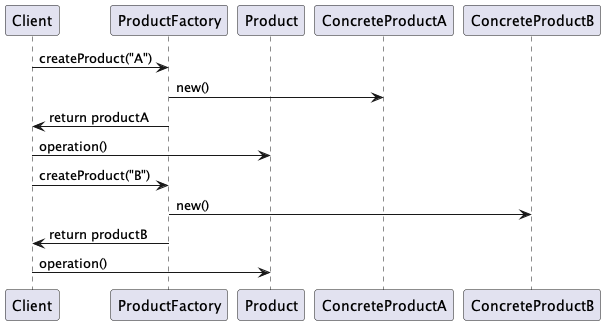
\includegraphics[width=0.85\textwidth]{fig/uml/factory-seq.png}
    \caption{Factory Pattern Sequenz}
    \label{fig:factory-seq}
  \end{figure}
\end{frame}

\begin{frame}
  \frametitle{Factory}
  \framesubtitle{Diskussion Eignung}
  \begin{itemize}
    \item Code sauberer und wartbarer
    \item Skalierbarkeit und Fehlertoleranz verbessert
    \item Viele Probleme bleiben: Kommunikationslatenz, Synchronisation, SPOF, Komplexität, Testbarkeit, Overhead
    \item Meist besser als Singleton
  \end{itemize}
\end{frame}
% ------------------------------------------------------------------------------
% Fin
\end{document}